% Created 2024-04-04 Thu 10:47
% Intended LaTeX compiler: pdflatex
\documentclass[presentation]{beamer}
\usepackage[utf8]{inputenc}
\usepackage[T1]{fontenc}
\usepackage{graphicx}
\usepackage{longtable}
\usepackage{wrapfig}
\usepackage{rotating}
\usepackage[normalem]{ulem}
\usepackage{amsmath}
\usepackage{amssymb}
\usepackage{capt-of}
\usepackage{hyperref}
\mode<beamer>{\usetheme{Madrid}}
\definecolor{SUred}{rgb}{0.59375, 0, 0.17969} % SU red (primary)
\definecolor{SUblue}{rgb}{0, 0.17578, 0.38281} % SU blue (secondary)
\setbeamercolor{palette primary}{bg=SUred,fg=white}
\setbeamercolor{palette secondary}{bg=SUblue,fg=white}
\setbeamercolor{palette tertiary}{bg=SUblue,fg=white}
\setbeamercolor{palette quaternary}{bg=SUblue,fg=white}
\setbeamercolor{structure}{fg=SUblue} % itemize, enumerate, etc
\setbeamercolor{section in toc}{fg=SUblue} % TOC sections
% Override palette coloring with secondary
\setbeamercolor{subsection in head/foot}{bg=SUblue,fg=white}
\setbeamercolor{date in head/foot}{bg=SUblue,fg=white}
\institute[SU]{Shenandoah University}
\titlegraphic{\includegraphics[width=0.5\textwidth]{\string~/Documents/suLogo/suLogo.pdf}}
\newcommand{\R}{\mathbb{R}}
\usepackage{tikz}
\usepackage{pgfplots}
\usetikzlibrary{calc}
\usetheme{default}
\author{Chase Mathison\thanks{cmathiso@su.edu}}
\date{5 April 2024}
\title{Law of Sines}
\hypersetup{
 pdfauthor={Chase Mathison},
 pdftitle={Law of Sines},
 pdfkeywords={},
 pdfsubject={},
 pdfcreator={Emacs 29.1 (Org mode 9.6.7)}, 
 pdflang={English}}
\begin{document}

\maketitle
\section{Announcements}
\label{sec:org3acf525}
\begin{frame}[label={sec:orgfa74445}]{Announcements}
\begin{enumerate}
\item Exam corrections due next Wednesday.
\item Homework in M.O.M.
\item Office hours today, 10am - 11am.
\end{enumerate}
\end{frame}

\section{Lecture}
\label{sec:org8cf8467}
\begin{frame}[label={sec:orgb390eeb}]{A few more advanced trig equation techniques}
Let's illustrate a few more ``advanced'' techniques for trig equations with the following examples on the interval \(0 \le \theta < 2\pi\):
\begin{enumerate}
\item \(2\sin^2(\theta) + \cos(\theta) = 2\)
\item \(2\sin(3\theta) = 1\)
\end{enumerate}

\vspace{10in}
\end{frame}

\begin{frame}[label={sec:org8b62a86}]{Example}
\end{frame}

\begin{frame}[label={sec:orgd3181a4}]{Law of Sines}
Let's look at a general \uline{\hspace*{1in}} and see what we can say about
it using right angle trigonometry.  We want to \uline{\hspace*{1in}} this
oblique triangle, which means finding all 3 \uline{\hspace*{1in}} and all 3 \uline{\hspace*{1in}}.

\begin{center}
\begin{tikzpicture}[scale=1.5]
  \node[left] at (0,0) {$A$};
  \node[right] at (3,0) {$B$};
  \node[above] at (2,2) {$C$};
  \draw (0,0) -- node[below] {$c$} (3,0) -- node[right] {$a$} (2,2) -- node[left] {$b$} cycle;
\end{tikzpicture}
\end{center}

\vspace{10in}
\end{frame}
\begin{frame}[label={sec:orgfe83703}]{Law of Sines}
We've just developed the Law of Sines!

\begin{theorem}[Law of Sines]
In any triangle with angles \(A,B,C\) and corresponding side lengths \(a,b,c\), we will always have:
\[
\frac{\sin(A)}{a} = \frac{\sin(B)}{b} = \frac{\sin(C)}{c}\]
\end{theorem}

Let's look at a few particular examples of how to use this!
\end{frame}
\begin{frame}[label={sec:orgf144174}]{ASA}
\begin{center}
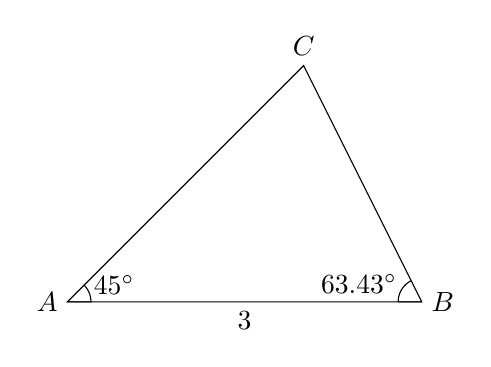
\begin{tikzpicture}[scale=1.5]
  \node[left] at (0,0) {$A$};
  \draw (0,0) -- ++(.2,0) arc (0:45:0.2);
  \node[right] at (45:0.2) {$45^{\circ}$};
  \node[right] at (3,0) {$B$};
  \draw (3,0) -- ++(-0.2,0) arc (180:116.57:0.2);
  \path (3,0) -- ++(130:0.2) node[left] {$63.43^{\circ}$};
  \node[above] at (2,2) {$C$};
  \draw (0,0) -- node[below] {$3$} (3,0) -- (2,2) -- cycle;
\end{tikzpicture}
\end{center}

\vspace{10in}
\end{frame}

\begin{frame}[label={sec:orga131918}]{AAS}
\begin{center}
  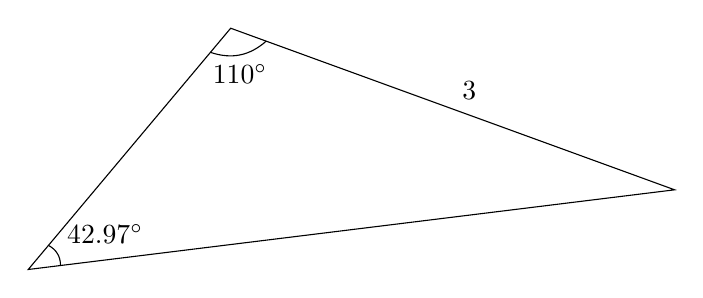
\begin{tikzpicture}[scale=2]
    \draw (0,0) coordinate (A) -- ++(50:2) coordinate (B) -- ++(-20:3) coordinate (C) -- cycle;
    \path (A) -- (B) -- node[above right] {$3$} (C);
    \draw[bend left] ($(A)!.1!(B)$) to node[above right] {$42.97^{\circ}$} ($(A)!.05!(C)$);
    \draw[bend right] ($(B)!.1!(A)$) to node[below] {$110^{\circ}$} ($(B)!.08!(C)$);
  \end{tikzpicture}
\end{center}

\vspace{10in}
\end{frame}

\begin{frame}[label={sec:orga1d1096}]{SSA}
\begin{center}
  \begin{tikzpicture}[scale=0.8]
    \draw (0,0) coordinate (A) -- node[above left] {$8$} ++(35:8) coordinate (B) -- node[right] {$6$} ++(-130.1:6) coordinate (C) -- cycle;
    \draw (A) -- ++(0.5,0) arc (0:35:0.5);
    \node[right] at (25:0.5) {$35^{\circ}$};
  \end{tikzpicture}
\end{center}

\vspace{10in}
\end{frame}

\begin{frame}[label={sec:orgf8c1b47}]{Examples}
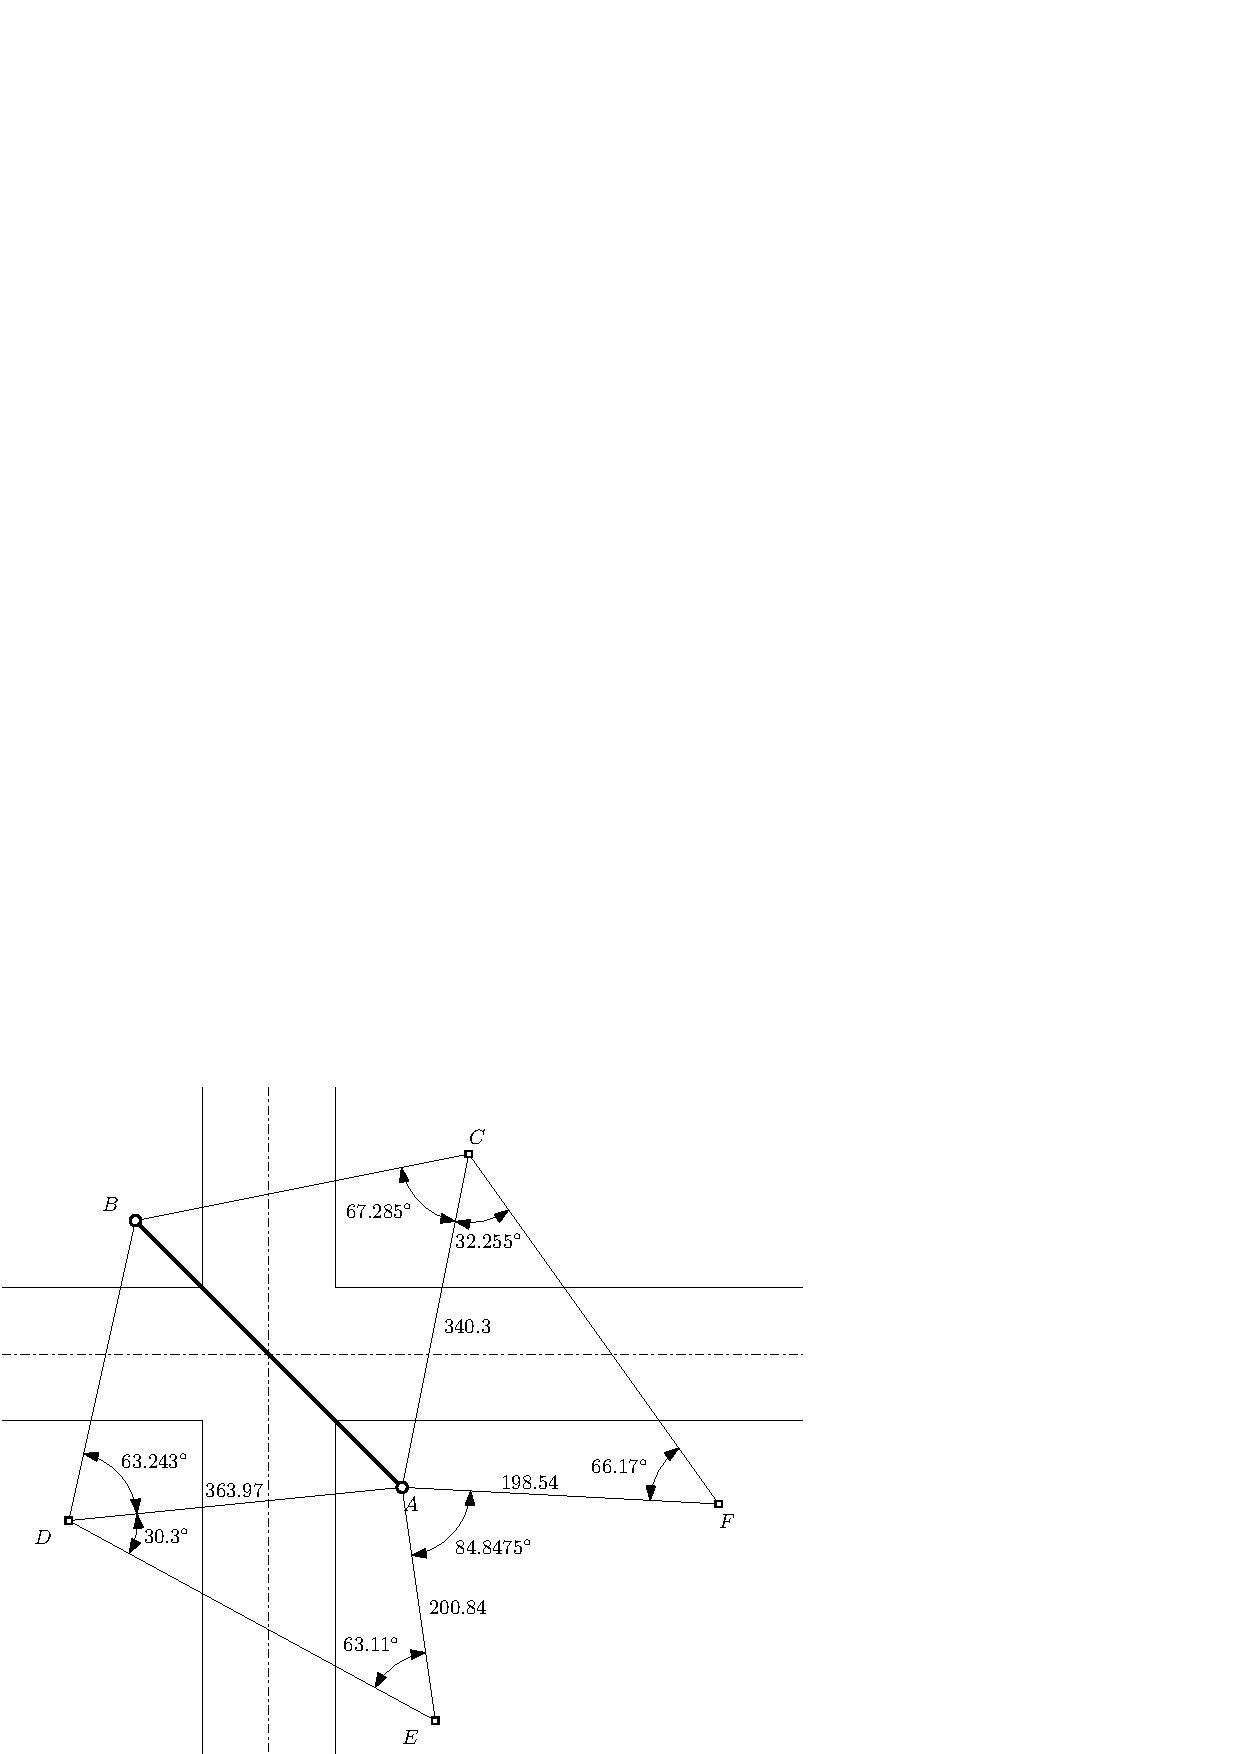
\includegraphics[height=0.8\textheight,trim=0in 0.6in 0in 1in, clip]{../trigStar.pdf}
\end{frame}
\end{document}